\section{Going further}

\begin{frame}{Debugging resources}
  \begin{itemize}
  \item Brendan Gregg
    \href{https://www.brendangregg.com/systems-performance-2nd-edition-book.html}{Systems
      performance} book
  \item Brendan Gregg
    \href{https://www.brendangregg.com/linuxperf.html}{Linux
      Performance} page
  \item {\em Tools and Techniques to Debug an Embedded Linux System},
    talk from Sergio Prado,
    \href{https://www.youtube.com/watch?v=dgPkZnGuIMg}{video},
    \href{https://elinux.org/images/c/cf/Slides-debugging.pdf}{slides}
  \item {\em Tracing with Ftrace: Critical Tooling for Linux
      Development}, talk from Steven Rostedt,
    \href{https://www.youtube.com/watch?v=mlxqpNvfvEQ}{video}
  \item {\em Tutorial: Debugging Embedded Devices using GDB}, tutorial
    from Chris Simmonds,
    \href{https://www.youtube.com/watch?v=JGhAgd2a_Ck}{video}
  \end{itemize}
\end{frame}

\begin{frame}[fragile]
  \frametitle{Going further (Tracing \& Profiling)}
  \begin{columns}
    \column{0.65\textwidth}
    \begin{itemize}
    \item Great book from Brendan Gregg, an expert in tracing and profiling
    \item https://www.brendangregg.com/blog/2020-07-15/systems-performance-2nd-edition.html
    \item Covers concepts, strategy, tools, and tuning for Linux kernel
      and applications.
    \end{itemize}
    \column{0.35\textwidth}
    
\includegraphics[height=0.6\textheight]{slides/debugging-system-wide-profiling/sysperf2nd_bookcover.png}\\ 
  \end{columns}
\end{frame}

\begin{frame}[fragile]
  \frametitle{Going further (BPF)}
  \begin{columns}
    \column{0.65\textwidth}
    \begin{itemize}
    \item Still from Brendan Gregg!
    \item Covers more than 150 tools that uses BPF.
    \item Explains how to analyze the results from these tools to optimize
      your system.
    \item https://www.brendangregg.com/bpf-performance-tools-book.html
    \end{itemize}
    \column{0.35\textwidth}
    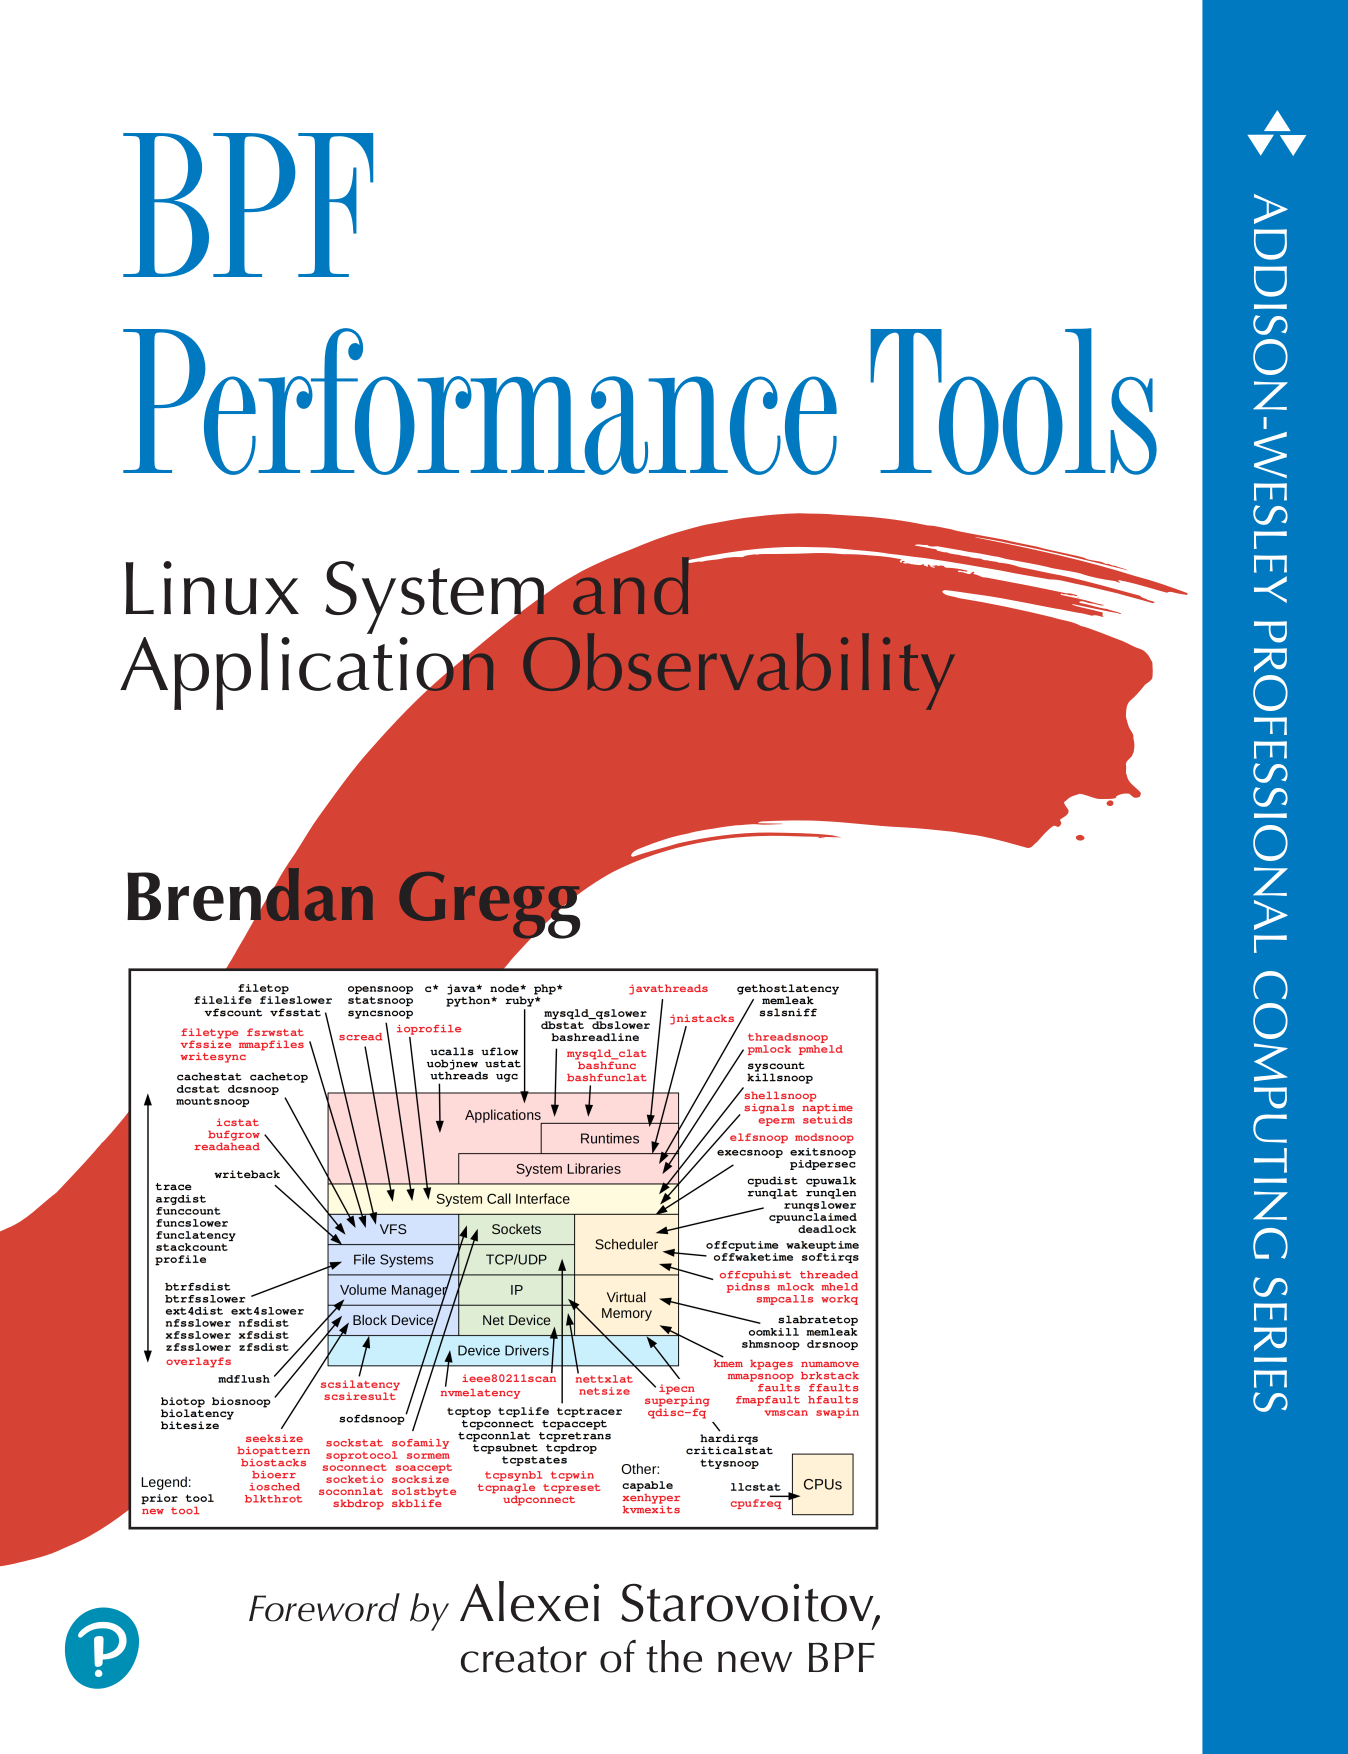
\includegraphics[height=0.6\textheight]{slides/debugging-system-wide-profiling/bpfperftools_bookcover.png}\\ 
  \end{columns}
\end{frame}